%
% kombiniert.tex -- Iterierte Kerne und Bilder
%
% (c) 2021 Prof Dr Andreas Müller, OST Ostschweizer Fachhochschule
%
\documentclass[tikz]{standalone}
\usepackage{amsmath}
\usepackage{times}
\usepackage{txfonts}
\usepackage{pgfplots}
\usepackage{csvsimple}
\usetikzlibrary{arrows,intersections,math}
\begin{document}
\definecolor{darkgreen}{rgb}{0,0.4,0}
\definecolor{turqoise}{rgb}{0,0.3,0.6}
\def\skala{1}
\newboolean{showgrid}
\setboolean{showgrid}{false}
\def\breite{7}
\def\hoehe{7}
\begin{tikzpicture}[>=latex,thick,scale=\skala]

\node at (0,0) {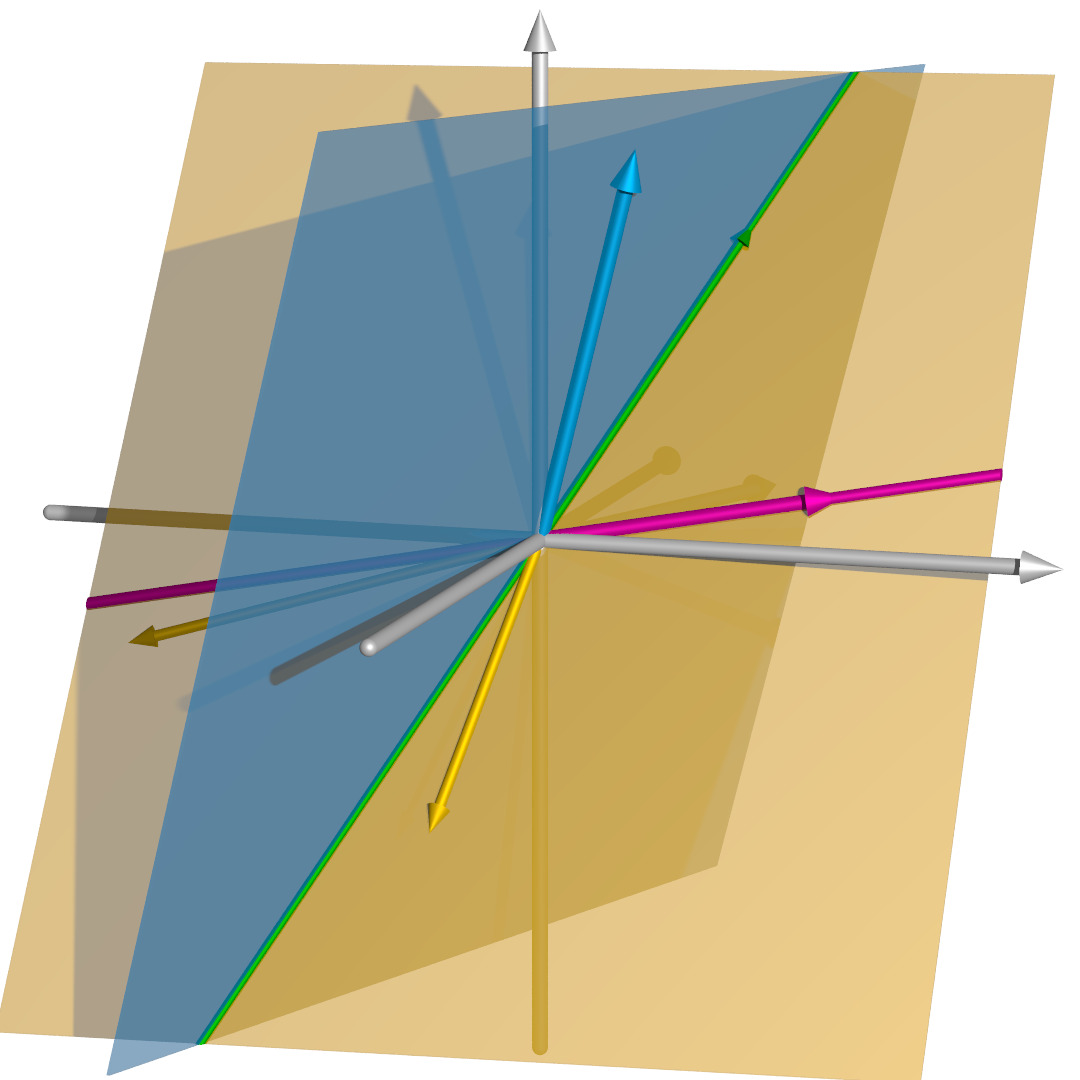
\includegraphics[width=13.8cm]{kombiniert.jpg}};

\node at (6.6,-0.1) {$x_1$};
\node at (0.3,6.7) {$x_3$};

\node[color=purple] at (4.8,1) [rotate=8] {$\mathcal{J}^2(A)$};
\node[color=darkgreen] at (3.5,4.6) [rotate=58] {$\mathcal{K}^1(A)$};

\fill[color=white,opacity=0.8] (-2.3,3.8) rectangle (-1.3,4.2);
\node[color=turqoise] at (-1.8,4) {$\mathcal{K}^2(A)$};

\fill[color=white,opacity=0.8] (2.5,-5.75) rectangle (3.5,-5.3);
\node[color=orange] at (3,-5.5) {$\mathcal{J}^1(A)$};

%\node at G
% Gitter
\ifthenelse{\boolean{showgrid}}{
\draw[step=0.1,line width=0.1pt] (-\breite,-\hoehe) grid (\breite, \hoehe);
\draw[step=0.5,line width=0.4pt] (-\breite,-\hoehe) grid (\breite, \hoehe);
\draw                            (-\breite,-\hoehe) grid (\breite, \hoehe);
\fill (0,0) circle[radius=0.05];
}{}

\end{tikzpicture}
\end{document}

